% Chapter Template

\chapter{Empirical Study} % Main chapter title

\label{Chapter5} % Change X to a consecutive number; for referencing this chapter elsewhere, use \ref{ChapterX}

%----------------------------------------------------------------------------------------
%	SECTION 1
%----------------------------------------------------------------------------------------
\section{Study Design}

As expected, para cumplir con el objetivo general de esta tesis se deben cumplir con los objetivos especificos, una vez estos sean completados a cabalidad entonces se tiene el objetivos general completado.

Explicar por qué se seleccionaron las herramientas (RIP, TestLab, etc)
Explicar las apps utilizadas en el estudio.

La idea es que estos objetivos especificos lleven o ayuden a llegar al cumplimiento de este objetivo general.

Se debe explicar cómo se cumplió con cada uno de ellos y al final explicar cómo se llegó a cumplir con el objetivo general

mostrar los resultados y analizarlos.

//TODO
two from the industry and two from the academic side. The first tool was Firebase Test Lab. it was selected for being widely used in industry and for also being a Google product. The second one, Monkey, was selected for being the most basic one and because it is also included in the SDK for developing Android Apps. The third one, Droidbot, was selected from the academic side. Droidbot has been a point of study for many researches. Many others tools have based their functionality on this tool. The last one is RIP, this tool was selected for being of special interest for us. It is our own exploration tool and is is currently an active project inside the Software Design Lab at University of Los Andes. 

Every tool was executed ten times per application, and every execution with a maximum time of 30 minutes. Some tools ended its exploration before the max time. 
The number of executions and the maximum time were arbitrary decisions that were made because of time limitations for the study. Although, during the study was notice that most of the tools ended the exploration or reached their maximum coverage within the first 15 minutes. Which means that the maximum time for exploration was more than enough in almost all cases. 
 



//TODO
Besides that, for this study, a set of 11 applications was used. This set is a subset of a set of open source applications utilised inside The Software Design Lab research group for other studies and tests, including RIP. Every APK in the subset should be successfully instrumented by InstruAPK, it should compile without any problem after instrumentation and it should be launch in an emulator without any issue after instrumentation.


\section{Context of the Study}

In order to present a fair comparison between MutAPK and MDroid+, we have used the same apps MDroid+ used for their experiments. This 54 applications presented in Table \ref{tab:alufs} belong to 16 different categories of the Google Play Store. It is worth noticing that these 54 applications are open source and allows us to study the way code statements are translated from JAVA to SMALI.

In order to collect data that allow us to answer the research question, we compared MutAPK to an existing tool for mutation testing that works at source code level ( MDroid+ \cite{linares2017enabling} ). 
The experiments were executed on a class-server machine. 
Note that in MutAPK, we implemented only 35 of 38 operators listed in Table \ref{tab:cmol} because the other 3 operators lead to non-compilable results. In order to analyze the impact of mutant generation process in MutAPK, we collect: (i) number of mutants generated per mutation operator per application; (ii) number of mutants that compile after mutation; (iii) mutant generation time (\textit{i.e.,} the time required to generate each mutant) and (iv) mutant building times (\textit{i.e.,} the time required to compile each APK file)
\begin{table}[t]
	\centering
	\caption{Applications used for the study}
	\label{tab:alufs}
	\resizebox{0.80\textwidth}{!}{
		\begin{tabular}{c c c c}
			App ID & Package Name & \# Methods Reported by APKAnalyzer & \# Methods Instrumented by InstruAPK\\
			\hline
			1 & appinventor.ai\_nels0n0s0ri0.MiRutina & 61993 & 9351\\
			2 & com.evancharlton.mileage & 4000 & 1162\\
			3 & com.fsck.k9 & 18799 & 7003\\
			4 & com.ichi2.anki & 32370 & 2209\\
			5 & com.workingagenda.devinettes & 19274 & 66 \\
			6 & de.vanitasvitae.enigmandroid & 13083 & 574 \\
			7 & info.guardianproject.ripple & 19429 & 100 \\
			8 & org.connectbot & 20606 & 1145\\
			9 & org.gnucash.android & 75473 & 504\\
			10 & org.libreoffice.impressremote & 14691 & 649\\
			11 & org.lumicall.android & 45784 & 540\\
			\hline
		\end{tabular}
	}
\end{table}

\begin{figure}[h]
\centering
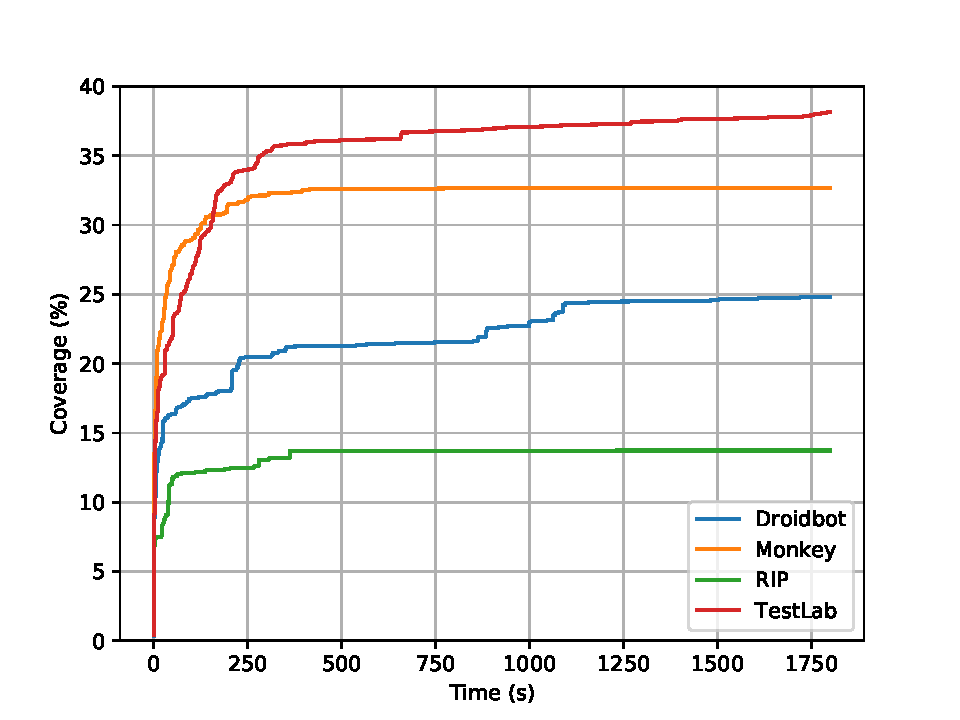
\includegraphics[width=0.8\textwidth]{../Figures/averageCoverageInstruAPK.pdf}
\caption{Average Method Coverage by Tool}\label{fig:averageCoverage}
\end{figure}

\begin{figure}[h]
\centering
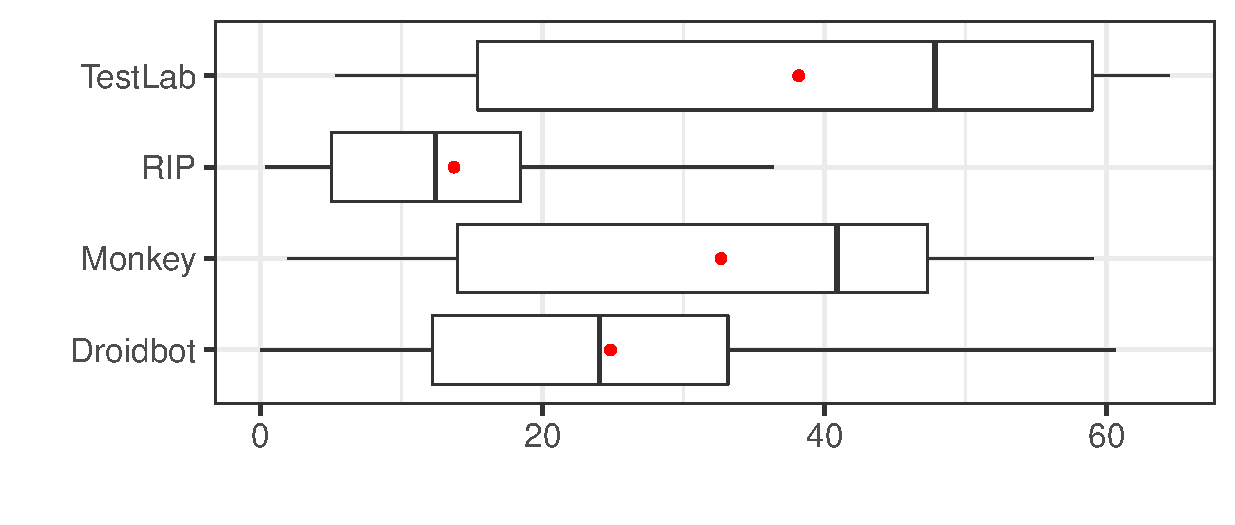
\includegraphics[width=0.8\textwidth]{../Figures/boxplotAccumulated.pdf}
\caption{Boxplot of Accumulated Coverage by Tool}\label{fig:boxplotAccumulated}
\end{figure}

\begin{figure}[h]
\centering
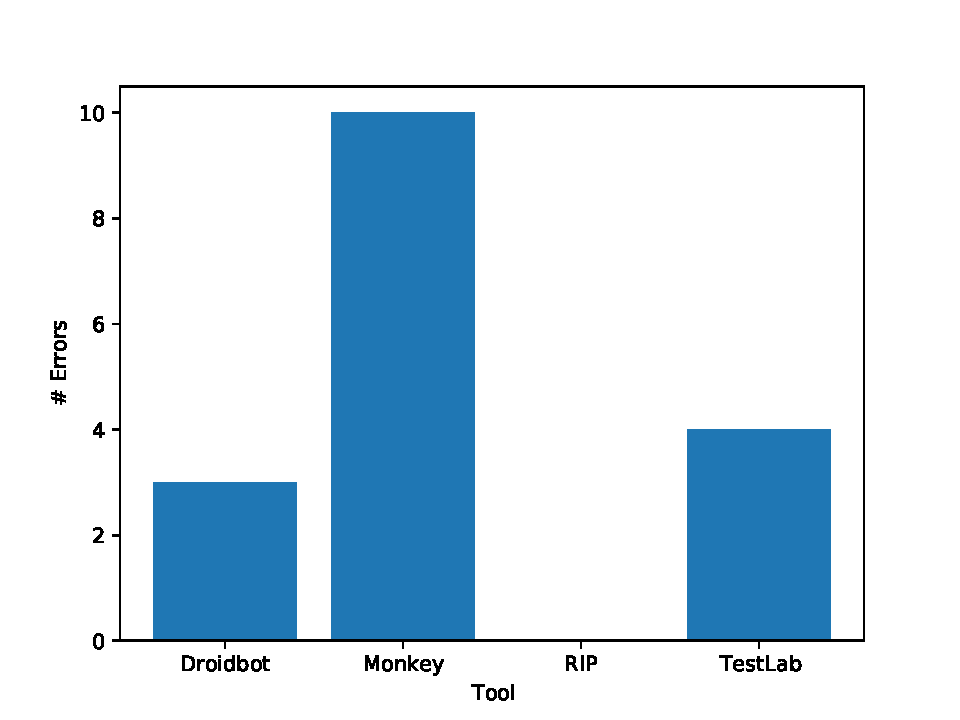
\includegraphics[width=0.8\textwidth]{../Figures/maxErrors.pdf}
\caption{Maximum Number of Errors Found by Tool}\label{fig:maxerrors}
\end{figure}

\begin{figure}[h]
\centering
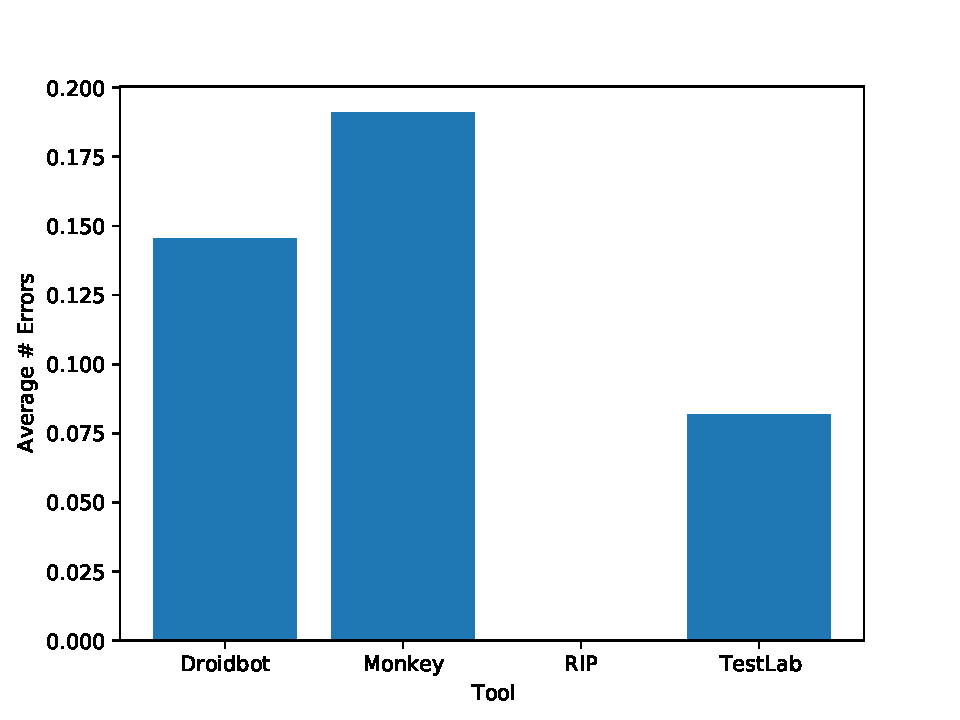
\includegraphics[width=0.8\textwidth]{../Figures/averageErrors.pdf}
\caption{Average Number of Errors Found by Tool}\label{fig:averagaerrors}
\end{figure}

\section{Results: Impact of generating mutants at APK level}

\textbf{\textit{$RQ_{1.1}$}}: To study our results, we present them in two stages, first we show a comparison where only the 33 mutants  in both MDroid+ and MutAPK are taken into account. In Figure \ref{fig:s22agmbp} we show the total amount of generated mutants per app. MutAPK generates around 30 more mutants per app (17\% more than MDroid+). However, if all operators are taken into account, the difference between the amount of mutants get bigger. Figure \ref{fig:agmbp} shows the amount of generated mutants per app. As it can be seen, MutAPK outperforms MDroid+ generating in average 1211 more mutants per app, this corresponds to 7.3 times more mutants. For further analysis of the results at app level, we added the Tables \ref{tab:cal1} and \ref{tab:cal2}, where all info collected is summarized around apps (See Appendix A). Also, we show in Figure \ref{fig:s22agmmobp} that the amount of mutants generated per mutant operator are very similar between MutAPK and MDroid+. It is worth nothing that this figure does not take into account the 63441 mutants generated by one of the operators implemented only in MutAPK. 

\textbf{\textit{$RQ_{1.2}$}}: If we consider again only the 33 shared mutants, in Figure \ref{fig:s22pncmbp} we can see that MutAPK generates around 16\% of non-compilable mutants while MDroid+ generates only 0.5\%. Nevertheless, when using all operators MutAPK generates around 2.36\% of non-compilable mutants while MDroid+ lightly increase its rate to 0.6\%. At the same time, Figure \ref{fig:s22pncmmobp} shows the percentage of non-compilable mutants in terms of the mutant operators, from this we can see that there is also a similar behavior for both. Specifically, MutAPK generates in average 0.1\% non-compilable mutants while MDroid generates 0.05\%.

\textbf{\textit{$RQ_{1.3}$}}: The most important result is the execution time. MutAPK takes only 3\% of the time ( 144,66ms ) required by MDroid+ ( 4,6 seconds) to mutate a copy of the app. Therefore, due to the infraestructure used to run our study, MutAPK takes 9 seconds to generate all mutants for an app (on average), while MDroid takes 19 seconds. 

\textbf{\textit{$RQ_{1.4}$}}: For compilation, MutAPK spends only 6.3\% of the time required by MDroid+ to compile a mutant. Consequently, MutAPK takes 11 min to compile all mutants for an app (on average) while MDroid+ takes 13 min.


Finally, if all mutant operators are selected, MutAPK takes around 9.63 hours to complete the mutation and compilation process for the 54 apps while MDroid+ takes 12 hours.  It is worth remembering that MutAPK generates around 7.3 times more mutants than MDroid+. Therefore, the remaining time could be used by developers,  practitioners, and servers to other software engineering activities. Additionally, as MutAPK generates more mutants, the generated search/bugs space  might be more comprehensive, which means that the quality of the test suite can be tested in a more wide sense.

\section{Analysis of non-compilable mutants}

In order to understand the reasons for non-compilable mutants, we analyzed 3 mutants for each one of the mutant operators that generated non-compilable. It is worth noting that this process must be iterative and after finding and fixing the errors, the mutation process must be executed again.

\subsection{31 - InvalidIDFindView}

This operator generated more non-compilable mutants than others. For this operator we found there is an implementation error when the mutation was performed. The correct implementation should be to include \textit{const <constVarName>, 0x<randomlyGeneratedHexa>} before the view was created to assign a random generated value to the key used as view ID. However, we injected \textit{const/16 <constVarName>, 0x<randomlyGeneratedHexa>} that generated a packaging error due to specific instructions that must accompanying \textit{const/16} and not \textit{const}.

After this error was fixed the percentage of non-compilable mutants at app level without taking into account non-shared operators decreases to 4\%.

\subsection{27 - FindViewByIdReturnsNull}

This operator presents two cases we did not consider. Listing \ref{lst:fvbirn1} presents the SMALI representation for finding an Android view; the mutation rule asks to convert the result of the search into a null object. Therefore, Listing \ref{lst:fvbirn2} presents the  SMALI instruction that must be injected instead of the previous one to assign a null value to the result. Nevertheless, after the mutation is performed when the compilation process is launched, an error is displayed on the console (Listing \ref{lst:fvbirn3}), saying that all available registers are between 0 and 15. After a deeper analysis, we found that registers after 16 inclusive are used only for referencing values and a null value could not be assigned. Therefore, we found that a cumbersome process most be made and a verification of the value of the 16th available register must be performed to save the value while the result of the mutation is used, and then the original value can be reassigned to the used register.

This behavior was found in several mutants.

We found that last line of Listing \ref{lst:fvbirn1} that is in charge of checking the type of the result, is not necessary and can be removed in some cases as it can be seen in Listing \ref{lst:fvbirn4} . Therefore, our implementation search for that instruction to recognize the complete set of instructions that will be replaced. Therefore, MutAPK throws an error when trying to match this expression with next line.

\subsection{4 - InvalidKeyIntentPutExtra}

Listing \ref{lst:ikipe} shows the result of executing the compilation process over half of the mutants from this mutation operator that are non-compilable. As it can be seen in the listing, the process ends succesfully but no apk file is generated. At this point we think that we might be facing an error within APKTool (\textit{i.e., the tool used for assembling/disassembling an APK}).

If these 4 mutant operators are updated and they do not generate non-compilable mutants, the percentage of non-compilable mutants at APK level (without taking into account the non-shared operators) should be dropped to 0.1\%.





